\chapter{Learning from scratch exploiting Robot Models}
\label{ch:learning_from_scratch}

In the previous chapter, we proposed a unified framework to develop robotic environments for \ac{RL} research.
The range of possible decision-making tasks that can be applied to robots is broad, from manipulation to locomotion.
This chapter considers the task of balancing the humanoid robot iCub in the presence of external disturbances in a simulated setting.
Framing the control objective as a \ac{RL} problem, we aim to train with the \ac{PPO} algorithm a policy encoded as a \ac{NN} capable of synthesising the appropriate instantaneous control signals of 23~\acp{DoF} of the iCub humanoid robot.
The resulting control action, simultaneously operating on both the upper- and lower-body joints, encodes multiple whole-body push-recovery strategies involving the usage of ankles, hips, momentum, and stepping strategies.
The policy automatically selects and blends all these different strategies upon need.

The presented architecture adopts a \emph{reward shaping} methodology that exploits as prior information quantities computed from the robot description, such as whole-body momentum and data related to the robot's \ac{CoM}.
This approach allows utilising the widely used family of model-free \ac{RL} algorithms while exploiting priors without changing the overall learning framework.
The priors act only as exploration hints, therefore, the model description does not need to be excessively accurate.
We also apply domain randomization over the model description used in simulation, resulting in differences between the simulated robot's dynamics and the model's dynamic from which the reward-shaping priors are computed.

\section{Training Environment}

\begin{figure}
    \centering
    \includegraphics{images/contributions/chapter_6/hierarchical_control_system.tikz}
    \caption{The proposed control system.}
    \label{fig:hierarchical}
\end{figure}

The decision-making logic is structured as a continuous control task with early termination conditions.
Its dynamics runs in the Gazebo Sim simulator embedded into the Gym-Ignition framework presented in Section~\ref{sec:gym_ignition}, exposing a \ac{RL} environment compatible with \verb|gym.Env|~\parencite{brockman_openai_2016}.
The enabled physics engine is DART~\parencite{lee_dart_2018}.
We selected iDynTree~\parencite{nori_icub_2015} for calculating rigid-body dynamics quantities that model the floating-base multibody system as described in Section~\ref{sec:multibody_dynamics}, whose dynamics is described by the following equation:
%
\begin{equation}
    M(\Qu) \Nud + h(\Qu, \Nu) = B \Torques + \sum_{L \in \mathcal{L}} J_{W,L}^\top(\Qu) \forcesix_L^{ext}
    .
\end{equation}
%
The iDynTree library allows to load a model description encoded in \ac{URDF} and provides all the terms forming this Lagrangian representation of the floating-base \acp{EoM} together with additional quantities that will be included in the reward computation described in Section~\ref{sec:reward_shaping}.

Figure~\ref{fig:hierarchical} reports a high-level overview of the proposed control system.
The environment receives actions from the agent, here represented as its underlying \ac{NN}, and produces observations and rewards at 25~Hz.
The physics and the low-level \pid controllers run at 1000~Hz.
During training, some properties of the environment are randomised (see Sec.~\ref{sec:env-other}).

\pagebreak
\subsection{Action}

The separation between agent and environment is defined by the  action selection.
In our nested structure, the policy generates an action $\mathbf{a} \in \mathbb{R}^{23}$ composed of the reference velocities for a large subset of the robot joints (controlled joints), which are then integrated and fed to the corresponding \pid position controllers.
The controlled joints belong to the legs, torso, and arms.
Hands, wrists, and neck, which arguably play a minor role in balancing, are locked in their natural positions.
The policy computes target joint velocities bounded in $[-180,180]$~deg/s at $25$~Hz.
Commanding joint velocities rather than joint positions prevents target joint positions from being too distant from each other in consecutive steps.
Especially at training onset, this would lead to jumpy references that the \pid controllers cannot track, affecting the discovery of the relation between the states $\mathbf{x}_t$ and $\mathbf{x}_{t+1}$.
The integration process, instead, enables to use a policy that generates discontinuous actions while maintaining continuous \pid inputs with no need for additional filters.

\subsection{State}

\begin{table}
    \small
    \center
    \caption{Observation components.}
    \label{tab:observation}
    \begin{tabular}{llcc}
        \toprule
        Name & Value & Set & Range \\
        \midrule \rowcolor{black!10}
        Joint positions & $\mathbf{o}_s = \boldsymbol{s}$ & $\mathbb{R}^n$ & $[\boldsymbol{s}_{lb}, \boldsymbol{s}_{ub}]$ \\
        Joint velocities & $\mathbf{o}_{\dot{s}} = \dot{\boldsymbol{s}}$ & $\mathbb{R}^n $ & $[-\pi, \pi]$ \\ \rowcolor{black!10}
        Base height & $\mathbf{o}_h = \boldsymbol{p}_B^z$ & $\mathbb{R}$ & $[0, 0.78]$ \\
        Base orientation & $\mathbf{o}_R = (\rho, \phi)_B$ & $\mathbb{R}^2$ & $[-2\pi, 2\pi]$ \\ \rowcolor{black!10}
        Contact configuration & $\mathbf{o}_c = (c_L, c_R)$ & $\{0, 1\}^2$ & - \\
        \ac{CoP} forces & $ \mathbf{o}_f = (f^{CoP}_L, f^{CoP}_R)$ & $\mathbb{R}^2$ & $[0, mg]$ \\ \rowcolor{black!10}
        Feet positions & $\mathbf{o}_F = ({}^B \boldsymbol{p}_L, {}^B \boldsymbol{p}_R)$ & $\mathbb{R}^6$ & $[0, 0.78]$ \\
        \ac{CoM} velocity & $\mathbf{o}_v = {}^{G}\boldsymbol{v}_{CoM}$ & $\mathbb{R}^3$ & $[0, 3]$ \\
        \bottomrule
    \end{tabular}
\end{table}

Since no perception is involved, the state of the \ac{MDP} contains information about the robot's kinematics and dynamics.
It is defined as the tuple $\mathbf{x} := \langle \mathbf{q}, \mathbf{\boldsymbol{\nu}}, \mathbf{f}_L, \mathbf{f}_R \rangle \in \mathcal{X}$, where $(\mathbf{f}_L, \mathbf{f}_R)$ are the 6D forces exchanged between the feet and the terrain.
The observation, computed from the state $\mathbf{x}$ and the robot model $\mathcal{M}$, is defined as the tuple
%
\begin{equation*}
    \boldsymbol{o} =
    \boldsymbol{o}(\mathbf{x}, \mathcal{M}) :=
    \langle \mathbf{o}_s, \mathbf{o}_{\dot{s}}, \mathbf{o}_h, \mathbf{o}_R, \mathbf{o}_c, \mathbf{o}_f, \mathbf{o}_F, \mathbf{o}_v \rangle \in \mathcal{O}
\end{equation*}
%
where $\mathcal{O} := \mathbb{R}^{62}$.
%
The observation consists of the following terms, each of them re-scaled\footnote{We also call the re-scaling operation of a bounded variable as \emph{normalization}.} into a given interval for better properties when used as \ac{NN} inputs:
%
\begin{itemize}
%
\item $\mathbf{o}_s$ are the controlled joints angles in radians, normalised with the hard limits defined in the model description; 
%
\item $\mathbf{o}_{\dot{s}}$ are the velocities of the controlled joints, normalised in $[-\pi, \pi]$~rad/s;
%
\item $\mathbf{o}_h$ is the height of the base frame, normalised in $[0, 0.78]$~m;
%
\item $\mathbf{o}_R$ is a tuple containing the roll and pitch angles of the base frame \wrt the world frame, normalised in $[-2\pi, 2\pi]$~rad;
%
\item $\mathbf{o}_c$ is a tuple defining whether the feet are in contact with the ground;
%
\item $\mathbf{o}_f$ is a tuple containing the vertical forces applied to the local \ac{CoP} of the feet (see Appendix~\ref{appendix:center_of_pressure} for its definition), normalised in $[0, 330]$~N, \ie the nominal weight force of the robot;
%
\item $\mathbf{o}_F$ is a tuple containing the positions of the feet \wrt the base frame, normalised in $[0, 0.78]$~m;
%
\item $\mathbf{o}_v$ is the linear velocity of the \ac{CoM} expressed in the \ac{CoM} frame $G = (\pos_{CoM}, [B])$, normalised in $[0, 3]$~m/s.
%
\end{itemize}
%
The exact definition of all the observation terms is reported in Table~\ref{tab:observation}.

Although the agent is trained in simulation, we design it for real-time execution on actual robots.
We carefully select state components that can be either measured or estimated on-board~\parencite{nori_icub_2015}.
To promote policy transfer, we avoid measurements from noisy sensors and values that cannot be estimated with sufficient accuracy.
In fact, any significant mismatch between simulated and real data would hinder transfer, increasing the reliance on policy robustness.
We select minimal state components encoding the environment dynamics without affecting learning performance.

\subsection{Other specifications}\label{sec:env-other}

\paragraph{Initial State Distribution}

The initial state distribution $\rho(\mathbf{x}_0): \mathcal{X} \to \mathcal{O}$ defines the value of the observation in which the agent begins each episode.
Sampling the initial state from a distribution with small variance, particularly regarding joint positions and velocities, positively affects exploration without degrading the learning performance.
At the beginning of each episode, for each joint $j \in \mathcal{J}$ we sample its position $s_{j,0}$ from $\mathcal{N}(\mu=s_0, \sigma=10 \, \text{deg})$, where $s_{0}$ represents the fixed initial reference, and its velocity $\dot{s}_{j,0}$ from $\mathcal{N}(\mu=0, \sigma=90 \, \text{deg/s})$.
As a result, the robot may or may not start with the feet in contact with the ground, encouraging the agent to learn how to land and deal with impacts.

\paragraph{Exploration}

In order to promote exploration beyond the initial state distribution and favour the emergence of push-recovery strategies, we apply external perturbations in the form of a 3D force to the robot's base frame located over its pelvis.
The applied force vector has a fixed magnitude of 200~N and is applied for 200~ms.
Considering the weight of the iCub, approximately 33~kg, the normalised impulse sums up to 1.21~Ns/Kg.
We sample the direction of the applied force from a uniform spherical distribution.
The frequency of the application is defined as average applications per second, again sampling from a uniform distribution.
We apply a force on average every 5 simulated seconds.

\paragraph{Early Termination}

The balancing and push-recovery objectives for a continuous-control task are characterised by an infinite-horizon discounted \ac{MDP}.
During training, however, episodes should stop as soon as the state reaches a subspace from which either it is impossible to recover or uninteresting to explore, following an early-termination criterion.
The state space interesting for our work is where the robot is -- almost -- standing on its feet, therefore we terminate the episodes as soon as it falls to the ground.
We detect the falling condition when any link but the feet touches the ground plane.

\paragraph{Domain Randomisation}

During the training process, the environment performs a domain randomisation step at the beginning of each new episode.
The masses of the robot's links are sampled from a normal distribution $\mathcal{N}(\mu=m_0, \sigma=0.2 m_0)$, where $m_0$ is the nominal mass of the link defined in the model description.
To avoid making assumptions about the feet's and ground's material properties, we randomise the Coulomb friction $\mu_c$ of the feet by sampling it from $\mathcal{U}(0.5, 3)$.
Finally, since the simulation does not include the real dynamics of the actuators, to increase robustness, we apply a delay to the position references fed to the \pid controllers, sampled from $\mathcal{U}(0, 20)$~ms, and kept constant during the entire episode (until termination).

\section{Agent}

\begin{table}
    \small
    \center
    \caption{PPO, policy, and training parameters.}
    \label{tab:training_parameters}
    \newcommand{\ck}{\checkmark}
    \begin{tabular}{cc}
        \toprule
        Parameter & \multicolumn{1}{c}{Value} \\
        \midrule \rowcolor{black!10}
        Discount rate $\gamma$ & 0.95 \\
        Clip parameter $\epsilon$ & 0.3 \\ \rowcolor{black!10}
        Learning rate $\alpha$ & 0.0001 \\ 
        GAE parameter $\lambda$ & 1.0 \\ \rowcolor{black!10}
        Batch size & 10000 \\ 
        Minibatch size & 512 \\ \rowcolor{black!10}
        Number of SGD epochs & 32 \\ 
        Number or parallel workers & 32 \\ \rowcolor{black!10}
        Value function clip parameter & 1000 \\ 
        \bottomrule
    \end{tabular}
\end{table}

The agent receives the observation $\boldsymbol{o}$ from the environment and returns the action $\mathbf{a}$ defining the reference velocities of the controlled joints.
The agent parameters are reported in Table~\ref{tab:training_parameters} and further explained below.

\paragraph{Learning Algorithm}

We select \ac{PPO} as the candidate learning algorithm, in the variant that includes both the clipped surrogate and \ac{KL} penalty objectives introduced in Section~\ref{sec:ppo}.
We selected this algorithm since it provides a simple but effective implementation of policy optimization, widely used in comparable studies\footnote{This chapter is mainly focused on the reward shaping process, not on the specific algorithm used to train the agent.}.
A practical benefit of \ac{PPO} is its small number of parameters (only the clip parameter $\epsilon$ if the \ac{KL} penalty coefficient is adjusted dynamically) that does not excessively overload the parameter tuning process.

\paragraph{Policy and Value Function}

The policy, given an observation $\boldsymbol{o}_t$, samples the action $\boldsymbol{a}_t$ to take from the stochastic distribution $\pi(\cdot \given \boldsymbol{o}_t)$.
The value function $\hat{V}(\boldsymbol{o}_t)$, instead, estimates the average return when starting from the observation $\boldsymbol{o}_t$ and then following the policy for the next steps.
We represent both the policy and the value function with two different neural networks composed of two fully connected layers, with 512 and 128 units each, followed by a linear output layer.
The hidden units use a ReLU activation function.
The networks do not share any layer.

\paragraph{Distributed Setup}

The chosen \ac{PPO} algorithm scales gracefully to a setup where the batch samples are collected from multiple workers in parallel.
A single trainer and 32 workers with an independent copy of the environment form our training setup.
After collecting a batch of 10000 on-policy transitions, we train the neural networks with stochastic gradient descent.
The optimiser uses mini-batches containing 512 samples and performs 32 epochs per batch.
The learning rate is $\lambda = 0.0001$.
Each trial is stopped once it reaches 20~M agent steps, roughly equivalent to 7~days of experience on a real robot.
Worker nodes run only on \ac{CPU} resources, while the trainer has access to the \ac{GPU} for accelerating the optimisation process.
We use the RLlib~\parencite{liang_rllib_2018} framework, OpenAI Gym, and distributed training.

\section{Reward Shaping}
\label{sec:reward_shaping}

\begin{sidewaystable}
    \center
    \caption{Reward function details. Terms with a defined cutoff are processed by the RBF kernel.}
    \label{tab:reward}
    \newcommand{\ck}{\checkmark}
    \setlength\extrarowheight{2pt}
    \begin{tabular}{lcrccrlrr}
        \toprule
        Name & Symbol(s) & Weight & Value $\mathbf{x}$ & Target $\mathbf{x}^*$ & \multicolumn{2}{c}{Cutoff $x_c$}  & SS & DS \\
        \midrule \rowcolor{black!10}
        Joint torques & $r_\tau$ & 5 & $\Vert \boldsymbol{\tau}_{step} \Vert $ & $\boldsymbol{0}_n$ & 10.0 & Nm & \ck & \ck \\
        Joint velocities & $r_{\dot{s}}$ & 2 & $\boldsymbol{a}$ & $\boldsymbol{0}_n$ & 1.0 & rad/s & \ck & \ck \\ \rowcolor{black!10}
        Postural & $r_{s}$ & 10 & $\boldsymbol{s}$ & $\boldsymbol{s}_0$ & 7.5 & deg & & \ck \\
        CoM $z$ velocity & $r_{v}^z$ & 2 & $\boldsymbol{v}^{xy}_{G}$ & $0$ & 1.0 & m/s & \ck & \ck \\ \rowcolor{black!10}
        CoM $xy$ velocity & $r_{v}^{xy}$ & 2 & $\boldsymbol{v}^{z}_{G}$ & $\omega_0 (\boldsymbol{p}^{xy}_{G} - \boldsymbol{\bar{p}}^{xy}_{hull})$ & 0.5 & m/s & & \ck \\
        Feet contact forces & $\{r_{f}^L, r_{f}^R\}$ & 4 & $\{f^{CoP}_L, f^{CoP}_R\}$ & $m g / 2$ & $m g / 2$ & N & \ck & \ck \\ \rowcolor{black!10}
        Centroidal momentum & $r_h$ & 1 & $\Vert {}_{G} \mathbf{h}_l \Vert^2 + \Vert {}_{G} \mathbf{h}_\omega \Vert^2$ & 0 & 50.0 & kg m$^2$/s & \ck & \ck \\
        Feet CoPs & $\{r_{p}^L, r_{p}^R\}$ & 20 & $\{\boldsymbol{p}_{L, CoP}, \boldsymbol{p}_{R, CoP}\}$ & $\{\bar{\boldsymbol{p}}^{xy}_{L, hull}, \bar{\boldsymbol{p}}^{xy}_{R, hull}\}$ & 0.3 & m & \ck & \ck \\ \rowcolor{black!10}
        Feet orientation & $\{r_{o}^L, r_{o}^R\}$ & 3 & $\{\mathbf{r}^{(z)}_L \cdot \mathbf{e}_z, \mathbf{r}^{(z)}_R \cdot \mathbf{e}_z\}$ & $1$ & 0.01 & - & \ck & \ck \\
        CoM projection & $r_{G}$ & 10 & $\boldsymbol{p}^{xy}_{G}$ & in the CH of support polygon & \multicolumn{1}{r}{-} & - & & \ck \\ \rowcolor{black!10}
        Feet in contact & $r_{c}$ & 2 & $c_L \land c_R$ & 1 & \multicolumn{1}{r}{-} & - & \ck & \ck \\
        Links in contact & $r_l$ & -10 & $c_{l}$ & $0$ & \multicolumn{1}{r}{-} & - & \ck & \ck \\
        \bottomrule
    \end{tabular}
\end{sidewaystable}

\subsection{RBF Kernel}

\ac{RBF} kernels are widely employed functions in machine learning, defined as
$$
K(\mathbf{x}, \mathbf{x}^*) = \exp \left( -\tilde\gamma ||\mathbf{x} - \mathbf{x}^*||^2  \right) \quad \in [0, 1] ,
$$
where $\tilde\gamma$ is the kernel bandwidth hyperparameter.
The \ac{RBF} kernel measures similarities between input vectors.
This can be useful for defining scaled reward components.
In particular, if $\mathbf{x}$ is the current measurement and $\mathbf{x}^*$ is the target, the kernel provides a normalised estimate of their similarity.
The variable $\tilde\gamma$ can be used to tune the bandwidth of the kernel, i.e.\ its sensitivity.
In particular, we use $\tilde\gamma$ to select the threshold from which the kernel tails begin to grow.
Introducing the pair $(x_c, \epsilon)$, with $x_c, \epsilon \in \mathbb{R}^+$ and $|\epsilon| \ll 1$, we can parameterise $\tilde\gamma = -\ln(\epsilon) / x_c^2$.
This formulation results in the following properties:

\begin{enumerate}
    \item $K(\mathbf{x}^*, \mathbf{x}^*) = 1$, i.e.\ when the measurement reaches the target, the kernel outputs 1;
    \item Given a measurement $\mathbf{x}_m$ such that $||\mathbf{x}_m - \mathbf{x}^*|| = x_c$, the kernel outputs $K(\mathbf{x}_m, \mathbf{x}^*) = \epsilon$.
\end{enumerate}

\noindent
In practice, $\epsilon$ can be kept constant for each reward component.
The sensitivity of individual components is tuned by adjusting $x_c$.
We refer to $x_c$ as \emph{cutoff} value of the kernel, since each norm of the distance in the input space bigger than $x_c$ yields output values smaller than $\epsilon$.
This formulation eases the composition of the total reward $r_t$ when reward components are calculated from measurements of different dimensionalities and scales.
In fact, once the sensitivities have been properly tuned for each component, they can simply be weighted differently as:
%
\begin{equation}
    \label{eq:weighted_reward_kernel}
    r_t = \sum_i w_i K \left( \mathbf{x}_i(t), \mathbf{x}_i^*(t) \right) \in \mathbb{R}
    ,
\end{equation}
%
where $\mathbf{x}_{i}(t)$ is the $i$-th measurement sampled at time $t$, and $w_i \in \mathbb{R}$ the weight corresponding to the $i$-th reward component.

\subsection{Reward}

This section describes all reward terms forming the instantaneous reward generated by the environment.
Given their number, we divided the terms in three categories: \emph{regularisers} are terms often used in optimal control for minimising the control action and the joint torques; \emph{steady-state terms} help obtain the balancing behaviour in the absence of external perturbations, and are active only in \ac{DS}; \emph{transient terms} favour the emergence of push-recovery whole-body strategies..
The logic of the task computes all reward terms at each environment step.
Then, all terms are processed with a \ac{RBF} kernel, weighted, and summed together using Equation~\eqref{eq:weighted_reward_kernel}, obtaining the final instantaneous reward $r_t$ returned to the agent for its maximisation during the training phase.

The situation in which all individual reward terms $r_i$ share the same range thanks to the filtering effect of the applied kernel simplifies the process of parameters tuning.
Each reward term introduces two parameters: its weight $\omega_i$ and the kernel cutoff $x_c$, where we assumed to keep the $\epsilon$ kernel parameter fixed.
Instead of applying grid-like search methods, that would require an excessively large number of permutations, we proceeded with an heuristic tuning by observing after each training the learning curve of each reward term independently.
Firstly, we tuned the cutoff parameter (\ie the sensitivity associated to the reward term) so that the agent could receive a perceivable increased reward to promote the desired exploration direction.
This process could be thought as tuning the variance of a Gaussian curve having mean over the target value.
Secondly, the reward terms with their tuned kernels are composed together by a weighted sum.
We started the tuning process from a weight of $1.0$ for all reward terms, and increased individual weights heuristically in case we wanted to adjust their relative importance.
Table~\ref{tab:reward} reports all the parameters of the reward function. 

\subsubsection{Regularisers}

\begin{description}

\item[Joint torques]\!($r_\tau$)\;
%
We compute the norm of all the joint torque references synthesised by the \pid controllers from the velocity references provided by the policy, and penalise this value.
The environment runs at 25~Hz and the low-level controllers at 1000~Hz.
Therefore, for each of the 23 joints, 40 torques are actuated between two consecutive environment steps.
We collect all these torques in a single vector $\boldsymbol{\tau}_{step} \in \mathbb{R}^{23\cdot40}$ and penalise its norm.

\item[Joint velocities]\!($r_{\dot{s}}$)\;
%
Our control scheme ensures that joint position references are continuous.
However, \ac{PPO} explores the action space of joint velocities following the active distributions.
To promote smoother trajectories, we penalise the norm of the latest action.
It can be seen as the minimisation of the control effort.

\end{description}

\subsubsection{Steady-state}

\begin{description}

\item[Postural]\!($r_s$)\;
%
Whole-body humanoid control schemes apply different weights to various control objectives.
The postural is notably one of the most used~\parencite{nava_stability_2016}, although it is usually assigned a low priority.
A postural reward term helps to reach a target posture during balancing instead of relying on local minima found in the learning process.
This component penalises the mismatch between the sampled joint configuration and the reference configuration shown in Figure~\ref{fig:icub_q0}.

\item[CoM projection]\!($r_{G}$)\;
%
Statically balanced robots, in order to maintain stability, keep the \ac{CoM} within the \ac{SP}, defined as the \ac{CH} of their contact points with the ground.
With the same aim, we introduce a Boolean component rewarding the agent if its \ac{CoM} ground projection is within the \ac{SP} induced by the feet.
For additional safety, we shrink the \ac{SP} by a 2.5~cm margin all along its perimeter.

\item[Horizontal CoM velocity]\!($r_{v}^{xy}$)\;
%
We define a target horizontal velocity for the \ac{CoM} as a vector pointing from the \ac{CoM} projection to the center of the \ac{SP} $\bar{\boldsymbol{p}}^{xy}_{hull}$.
In order to promote faster motions if the \ac{CoM} is relatively close to the ground, the magnitude of the target is amplified by a factor $w_0 = \sqrt{g / \boldsymbol{p}^z_{G}}$ derived from the \ac{LIP} model~\parencite{kajita_3d_2001}, where $g$ is the standard gravity.
This component encourages the motion of the \ac{CoM} projection towards the center of the \ac{SP}.

\end{description}

\subsubsection{Transient}

\begin{description}

\item[Feet in contact]\!($r_c$)\;
%
The feet are encouraged to stay on the ground.
In order to promote steps and increase movement freedom, we add a Boolean term marking whether any foot is in contact with the ground.

\item[Links in contact]\!($r_l$)\;
%
If any link excluding feet is in contact with the ground, the episode terminates with a negative reward of $-10$ for the terminal state.

\item[Whole-body momentum]\!($r_h$)\;
%
Our policy also controls joints belonging to the torso and the arms.
Therefore, the momentum generated by the upper body can be exploited for balancing and push recovery.
This term minimises the sum of the norms of the linear and angular components of the robot's total centroidal momentum ${}_G \mathbf{h}$~\parencite{traversaro_unied_2017}.

\item[Feet contact forces]\!($r_f$)\;
%
This reward term pushes the transient towards a steady-state pose in which the vertical forces at feet's \acp{CoP} $(f^{CoP}_L, f^{CoP}_R)$ (see Appendix~\ref{appendix:center_of_pressure}) assume the value of half of the robot's weight, distributing it equally on the two feet.

\item[Feet CoP]\!($r_p$)\;
%
Beyond the force at the feet \acp{CoP}, we also promote their positions to be located at the center of the corresponding sole $\bar{\boldsymbol{p}}^{xy}_{foot, hull}$.

\item[Vertical CoM velocity]\!($r_{v}^z$)\;
%
This reward component discourages vertical motion of the \ac{CoM} of the base link, promoting the usage of the horizontal component instead.

\item[Feet orientation]\!($r_o$)\;
%
In early experiments, the policy was converging towards feet tipping behaviours, i.e.\ the feet were not in full contact with the ground.
Since the terrain is flat by assumption, we discourage tipping by promoting a foot's orientation such that its sole is parallel to the ground.
If ${}^W R_{foot} = [\mathbf{r}^{(x)}, \mathbf{r}^{(y)}, \mathbf{r}^{(z)}]$ is the rotation between the foot frame and the world, this term promotes the alignment of its third column with the world frame.

\end{description}


\section{Results}

\subsection{Training performance}

Fig.~\ref{fig:learning_curves} reports the learning curves of the average reward and episode duration over 11 independent agent training runs.
Average reward across trials exhibits consistent growth and low variance (Fig.~\ref{fig:learning_curves}, left).
We have also observed increasing values for all individual reward elements during training.
Episode duration improves as well across trials and displays low variance (see Fig.~\ref{fig:learning_curves}, right), approaching maximum episode length more frequently as training progresses.

\begin{figure}
    \centering
    \resizebox{.85\textwidth}{!}{\includegraphics{images/contributions/chapter_6/learning_curves.tikz}}
    \caption{Learning curves over 11 training runs.}
    \label{fig:learning_curves}
\end{figure}

\subsection{Emerging behaviours}

Controlling the upper body enables rich recovery behaviours that involve the control of the total momentum of the kinematic structure.
We succeed in triggering such behaviours by applying external forces during policy training.
To make force profiles more realistic, we throw high-speed objects towards the balanced robot instead of applying constant forces for a fixed interval as done during training.
Figure~\ref{fig:sequences} shows two characteristic sequences.
A larger variety of push-recovery strategies are displayed in the following video: \url{https://ami-iit.github.io/emergence-push-recovery-icub}.

\subsection{Deterministic planar forces}

We evaluate the push-recovery performance by assessing the resilience from the application of external forces to the horizontal transverse plane of the robot.
Forces are applied for 0.2~s after 3~s from the simulation start, when the robot is stably standing still and front-facing.
Success is defined if the robot is still standing after 7~s, defining as a standing state the configuration in which only the feet can be in contact with the ground.
In Fig.~\ref{fig:force_polar}, success rates for forces pointing in 12 directions are reported.
Magnitudes increase from 50~N to 700~N at 25~N intervals.
Five repetitions are performed for each magnitude and direction, randomising the initial joints configuration by adding zero-mean Gaussian noise ($\sigma = 2$~deg).
Magnitudes within the training range (0-200~N) are counteracted successfully.
Remarkably, the policy is also robust to out-of-sample forces in all directions in (200-300~N), up to 400~N in some directions.
Moreover, it successfully recovers from pushes in the training range (0-200 N) even with an out-of-sample test friction coefficient $\mu_c=0.2$ (Fig.~\ref{fig:force_polar_low_friction}).

\begin{figure}
    \centering
    \hspace{-7mm}
    \subfloat[]{
        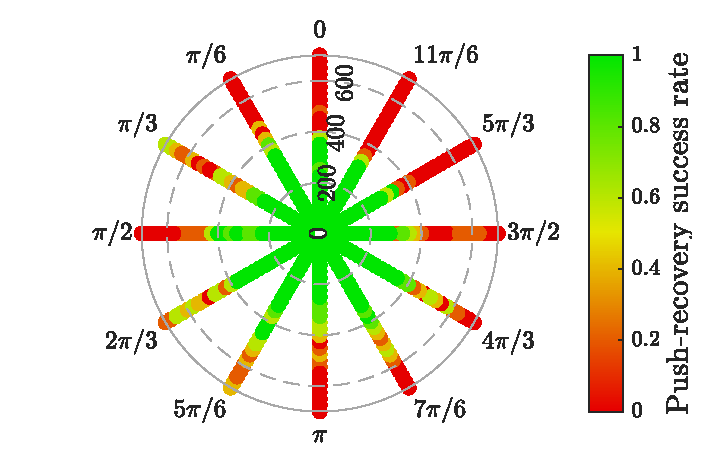
\includegraphics[width=0.5\textwidth]{images/contributions/chapter_6/results_polar_pi_frac_2_5rep_range50_700_25_rand_v3_adjusted.eps}
        \label{fig:force_polar}
    }
    \subfloat[]{
        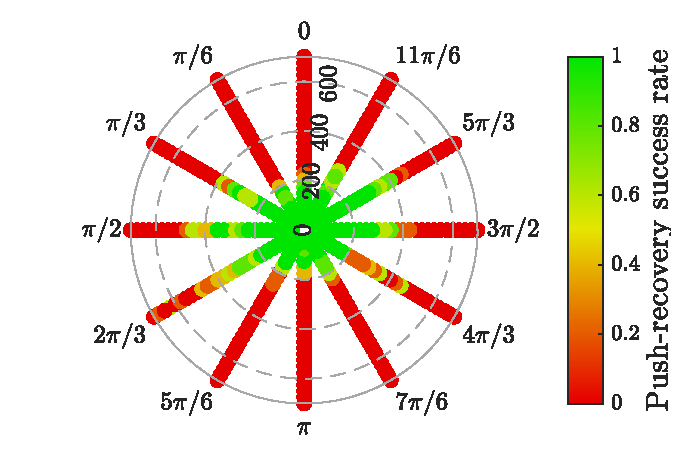
\includegraphics[width=0.5\textwidth]{images/contributions/chapter_6/results_final_policy_20M_polar_pi_frac_6_5rep_range50_700_25_rand_q_2deg_mu_0_2_v3_adjusted.eps}
        \label{fig:force_polar_low_friction}
    }
    \caption{(a)~Push-recovery success rates on the horizontal plane (forward push: $0$~rad, $\mu_c=1$). (b)~Results with  $\mu_c=0.2$.}
\end{figure}

\begin{figure}
    \centering
    \hspace{-3mm}
    \subfloat[]{
        \includegraphics[height=2.7cm]{images/contributions/chapter_6/icub_q0.jpeg}
        \label{fig:icub_q0}
    }
    \subfloat[]{
        \includegraphics[height=2.7cm]{images/contributions/chapter_6/sequences_highlight.png}
        \label{fig:sequences}
    }
    \caption{(a) The initial joint configuration $\boldsymbol{s}_0$. (b) Sequences showing ankle, step, and momentum push-recovery strategies. The robot is pushed by a sphere shot from the left side of the image. Impact takes place in the second frame.}
    \label{fig:q0_and_sequences}
\end{figure}

\subsection{Random spherical forces on the base links}

We evaluate policy robustness in challenging scenarios involving sequences of random forces with different combinations of magnitude and duration.
Forces are applied to the base in a random direction more frequently than during training, on average every 3~s.
For each combination, 50 reproducible episodes with different seed initialisation and no domain randomisation are executed.
Episodes terminate if the robot falls or after 60~s, averaging 20 applications in a complete episode.
Our evaluation metric is the number of consecutive forces endured by the robot.
Fig.~\ref{fig:random_forces} reports aggregate results for each combination of magnitude and duration.
No matter their magnitude, forces lasting 0.1~s are appropriately balanced.
As expected, performances decrease with growing magnitude and duration.
Nevertheless, the agent can withstand repeated applications of out-of-sample forces.
For instance, on average, it withstands 9 consecutive 300~N 0.2~s applications.

\subsection{Random spherical forces on the chest and elbow links}

We also evaluate the robustness of the learned policy to previously unseen forces applied to other links.
Fig.~\ref{fig:random_forces} shows the results obtained on the chest and elbow links.
As expected, forces applied on links that are far from the \ac{CoM} turn out to be more challenging.
Nevertheless, the policy is able to withstand a good number of them and generalise with good performances.
For instance, it is on average able to recover from 10 consecutive 200~N 0.2~s forces on the elbow link, as opposed to an average of 17 for the base link.
The average number of consecutive counterbalanced forces with the same magnitude and duration decreases to 5 for the chest link.
Notice that the randomness of the interval between two subsequent forces applications sometimes leads to challenging scenarios in which multiple forces are applied in a short time window.

\begin{figure}
    \centering
    \scriptsize
    \includegraphics[height=3.5cm,width=\textwidth]{images/contributions/chapter_6/forces_base.tikz}
    \includegraphics[height=3.5cm,width=\textwidth]{images/contributions/chapter_6/forces_chest.tikz}
    \includegraphics[height=4.7cm,width=\textwidth]{images/contributions/chapter_6/forces_elbow.tikz}
    \caption{Consecutive counterbalanced forces in random directions over 50 trials for each combination of magnitude and duration. Forces are applied to the base, chest, and elbow links for an increasing duration.}
    \label{fig:random_forces}
\end{figure}

\section{Conclusions}

In this chapter, we presented a control system composed of a high-level policy trained with \ac{RL} generating joint references actuated by low-level \pid controllers.
The system operates on the humanoid robot iCub with the aim of providing push-recovery capabilities in the presence of external disturbances.
We trained the \ac{RL} policy with the model-free \ac{PPO} algorithm.
In order to balance the exploration-exploitation trade-off and guide the training towards the desired behaviour, we relied on a careful reward shaping process that integrates into the reward signal returned by the environment multiple terms computed from the robot description acting as a prior.
We have shown that the resulting policy, operating on most of the joints of the iCub robot, is able to withstand repeated applications of strong external disturbances.
Depending on the magnitude of the disturbance, and the state of the system, the policy adopts different push-recovery strategies that include the usage of ankles, hips, stepping, and momentum.

The learning pipeline described in this chapter presents different limitations and shortcomings.
First, the training process to obtain a single policy requires an experience equivalent to approximately 7 simulated days, which is not surprising considering the low sample-efficiency typical of model-free \ac{RL} algorithms based on policy gradient.
Two possible ways to mitigate this problem are either switching to algorithms with better sample-efficiency, or optimising the performance of the experience generation.
The execution of the 7 simulated days, on a powerful workstation able to run 32 parallel simulations, lasts more than 2 real-world days, resulting in a long and extenuating parameters tuning process.
A second limitation comes from the chosen low-level control architecture, composed of independent \pid controllers.
Despite the benefits of their simplicity, they introduce in the system a stiffness that can prevent the emergence of natural and more human-like motions.
Finally, the applicability to real robots has yet to be assessed, since the simulation does not take into account second-order dynamic effects characterising real systems.
We tried to increase the robustness of the resulting policy by introducing multiple domain randomisation effects, but their effectiveness in the real world has not been assessed.
